% Bagian Tugas Modul
\section*{Tugas Modul} % Jika ada Tugas Modul
\begin{enumerate}
  \item Buatlah topologi jaringan percobaan 1, 2, dan 3!
      \begin{enumerate}
          \item Topologi 1: Point-to-Point
          \begin{figure}[htb]
            \centering
            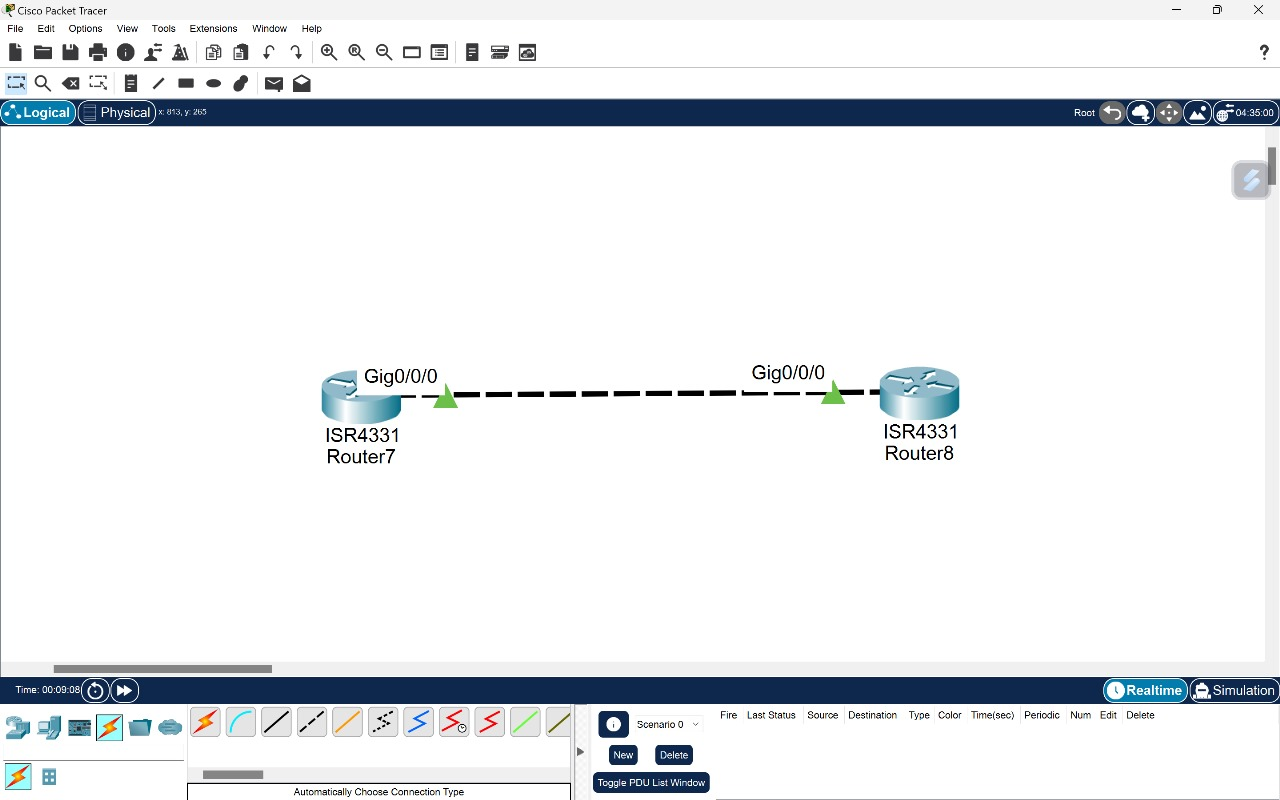
\includegraphics[width=0.7\textwidth]{img/point-point.jpeg}
            \caption{Topologi Point-to-Point}
            \label{fig:topo1}
          \end{figure}
          \item Topologi 2: Point-to-Multipoint
          \begin{figure}[htb]
            \centering
            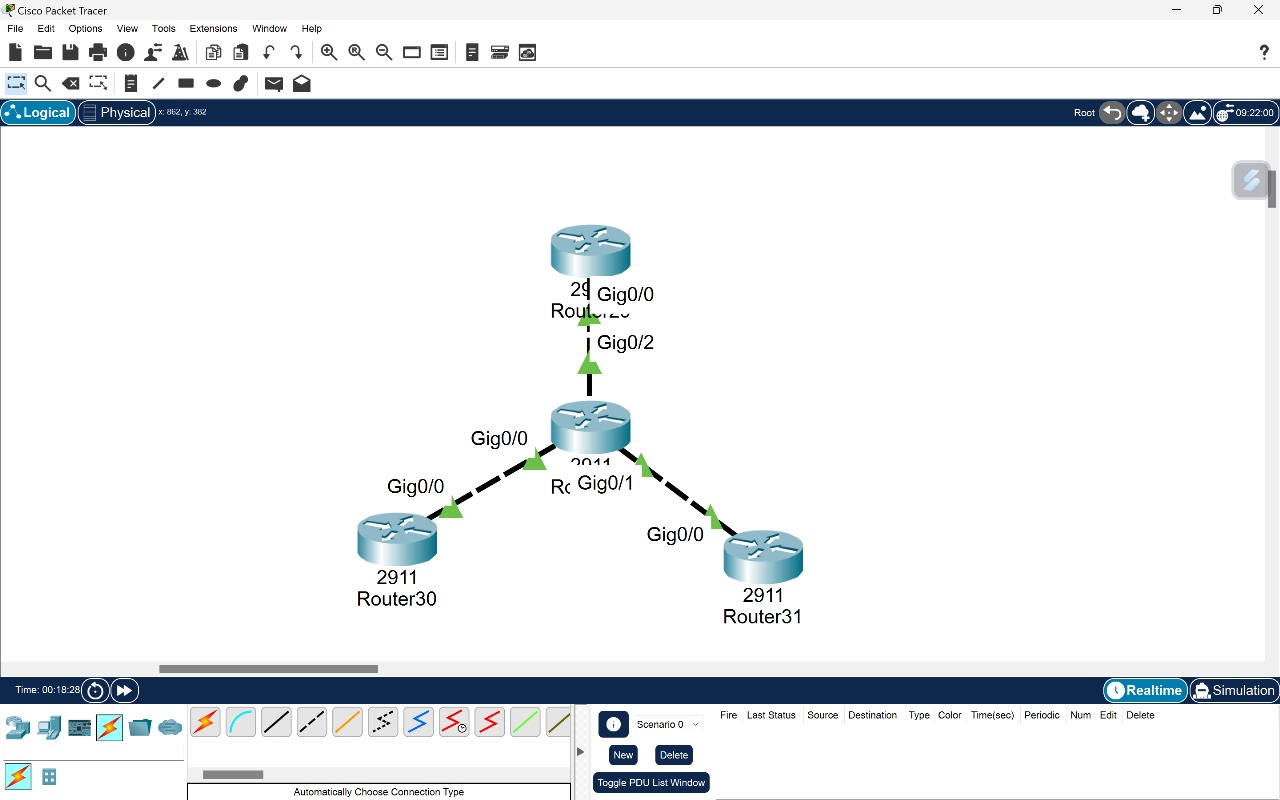
\includegraphics[width=0.7\textwidth]{img/point-multipoint.jpeg}
            \caption{Topologi Point-to-Multipoint}
            \label{fig:topo2}
          \end{figure}
          \item Topologi 3: Wireless Bridging
          \begin{figure}[htb]
            \centering
            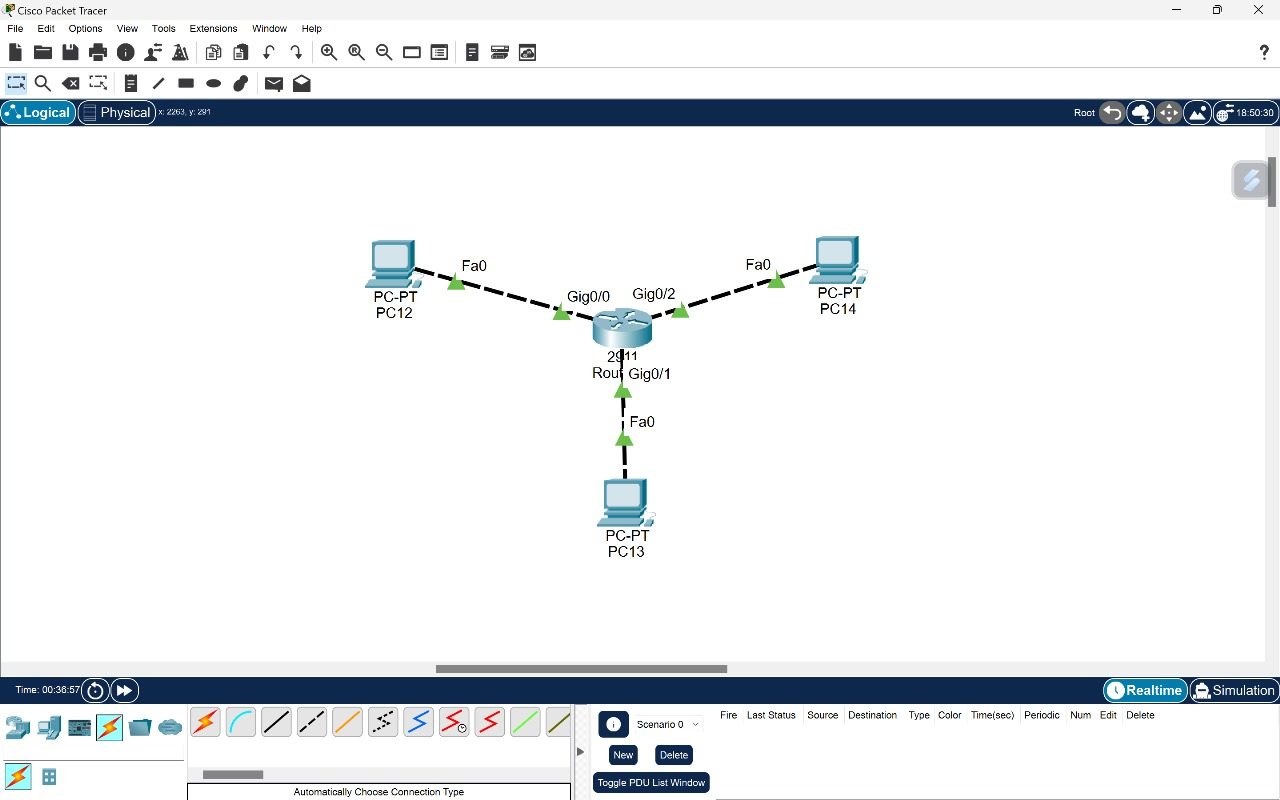
\includegraphics[width=0.7\textwidth]{img/wireless-bridging.jpeg}
            \caption{Topologi Wireless Bridging}
            \label{fig:topo3}
          \end{figure}
      \end{enumerate}
  \item Perbedaan Point-to-Point, Point-to-Multipoint, dan Wireless Bridging!
        
  \item Follow IG Lab MIOT ITS dan DM kami di @labmiotits dan @dm\_lab!
  
  Berikut ini adalah bukti kami telah mengikuti akun tersebut pada gambar \ref{fig:ig}:

  \begin{figure}[H]
    \centering
    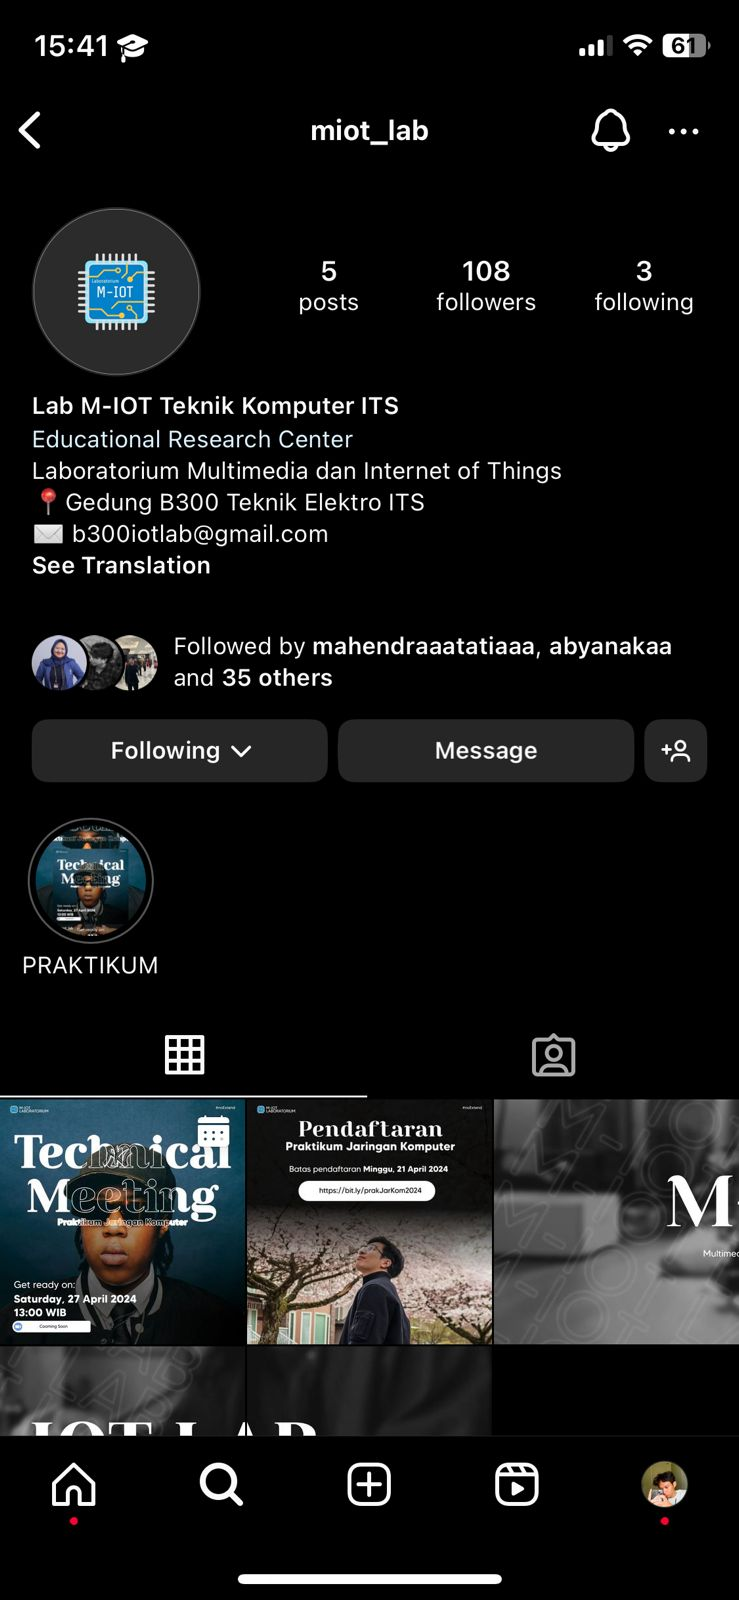
\includegraphics[width=0.5\textwidth]{img/ss_follow_b3.jpeg}
    \caption{Bukti Follow IG}
    \label{fig:ig}
  \end{figure}
        
\end{enumerate}